\section{Aufbau des Projekts}

Das Projekt hat die folgende Datei- und Ordnerstruktur:

\begin{figure}[H]
    \centering
    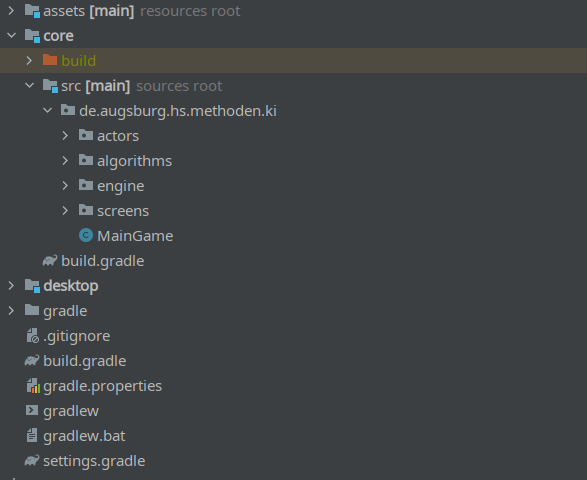
\includegraphics[width=0.6\textwidth]{figures/kap15/project-structure.png}
    \caption{Projektaufbau}
    \label{fig:prject-structure}
\end{figure}

\paragraph{MainGame class}

Die Klasse MainGame wird von der Funktion main (in desktop/src/de.augsburg.hs.methoden.ki\\.DesktopLauncher) instanziert und erweitert die Klasse ``Game'' von LibGDX. Die MainGame-Klasse dient als Einstiegspunkt f�r den Rest des Projekts.

\paragraph{Das ``actors'' Package}

``Actors'' bezieht sich auf Objekte, die von der Spiel-Engine verwaltet werden. Alle relevanten Akteure dieses Projekts sind hier zu finden.

\paragraph{Das ``algorithms'' Package}

Dieser Ordner enth�lt die Implementierungen der Algorithmen. Diese Implementierungen werden in ihren jeweiligen Kapiteln vorgestellt.

\paragraph{Das ``engine'' Package}

Dieser Ordner enth�lt den Code, der nicht direkt an der Implementierung der Algorithmen beteiligt ist, sondern als Basisklassen an die Implementierungen vererbt wird.

\paragraph{Das ``screens'' Package}

Ein ``Screen'' verweist auf verschiedene Levels im Spiel. F�r dieses Projekt ist jedes implementierte Vertiefungsprojekt in einem eigenen Screen enthalten.